\documentclass[a4paper,12pt]{article}
\usepackage[T2A]{fontenc}
\sloppy
\usepackage[utf8]{inputenc}
\usepackage[T2A]{fontenc}
\usepackage{babel}
\usepackage[a4paper,
left=2cm,
right=2cm,
top=2cm,
bottom=2cm]{geometry}
\usepackage{color}
\usepackage{mathtools}
\usepackage{listings}
\usepackage{graphicx}
\usepackage{tocloft}
\usepackage{indentfirst}
\usepackage{enumitem}
\usepackage{hyperref}

\setlength{\parindent}{0.8cm}
\setlength{\parskip}{0.4cm}
\renewcommand{\contentsname}{}
\renewcommand{\cftsecleader}{\cftdotfill{\cftdotsep}}
\renewcommand\refname{Список литературы}
\definecolor{dkgreen}{rgb}{0,0.6,0}
\definecolor{gray}{rgb}{0.5,0.5,0.5}
\definecolor{mauve}{rgb}{0.58,0,0.82}

\usepackage{caption} %заголовки плавающих объектов
\captionsetup[figure]{name=Рис} 

%Псевдокодик
\usepackage{algorithm}
\usepackage{algpseudocode}
\floatname{algorithm}{Алгоритм}

%C++ code 
\usepackage{listings}
\usepackage{color}
% параметры стиля
\lstdefinestyle{mystyle}{
	basicstyle=\footnotesize,
	breakatwhitespace=false, 
	breaklines=true,
	captionpos=b,
	keepspaces=true, 
	numbers=left,
	numbersep=5pt,  % номера строк
	showspaces=false, % не показывать пробелы
	showstringspaces=false,
	showtabs=false,                  
	tabsize=2
}

% применяем стиль
\lstset{style=mystyle}
% используем заданный нами моноширинный шрифт
\lstset{basicstyle=\footnotesize\ttfamily,breaklines=true}


\begin{document}
\begin{titlepage}
	\begin{center}
		\large
		{МИНИСТЕРСТВО НАУКИ И ВЫСШЕГО ОБРАЗОВАНИЯ\\ РОССИЙСКОЙ ФЕДЕРАЦИИ}
		
		Федеральное государственное автономное образовательное учреждение высшего образования
		\vspace{0.5cm}
		
		\textbf{<<Национальный исследовательский Нижегородский государственный университет им. Н.И. Лобачевского>>}\\
		(ННГУ)\\
		\vspace{1cm}
		\textbf{Институт информационных технологий, математики и механики}\\
		\vfill
		
		\Large
		ОТЧЕТ ПО ЛАБОРАТОРНОЙ РАБОТЕ\\
		на тему:\\
		\textbf{<<Повышение контраста полутонового изображения посредством 
линейной растяжки гистограммы.>>}
		{\LARGE 
		}
		\bigskip
		
		
	\end{center}
	\vfill
	
	\newlength{\ML}
	\settowidth{\ML}{«\underline{\hspace{0.7cm}}» \underline{\hspace{2cm}}}
	\hfill\begin{minipage}{0.4\textwidth}
		\textbf{Выполнил:}\\
		студент группы 3821Б1ФИ3\\
		\underline{\hspace{3cm}} Кузнецов А.А.\\
	\end{minipage}%
	\bigskip
	
	\hfill\begin{minipage}{0.4\textwidth}
		\textbf{Преподаватель:}\\
		\underline{\hspace{3cm}} Нестеров А.Ю. \\
	\end{minipage}%
	\vfill
	
	\begin{center}
		Нижний Новгород\\
		2023 г.
	\end{center}
\end{titlepage}

\thispagestyle{empty} % убираем колонтитулы с этой страницы

\tableofcontents
\newpage

\section*{Введение}
\addcontentsline{toc}{section}{Введение}
Один из наиболее распространенных дефектов фотографических, сканерных и телевизионных изображений – слабый контраст. Дефект во многом обусловлен ограниченностью диапазона воспроизводимых яркостей. Под контрастом понимается разность максимального и минимального значений яркости. Контрастность изображения можно повысить за счет изменения яркости каждого элемента изображения и увеличения диапазона яркостей. Существует несколько методов, основанных на вычислении гистограммы. В данной лабораторной работе будет рассматриваться алгоритм \textbf{линейного растяжения гистограммы}.

\section*{Постановка задачи}
\addcontentsline{toc}{section}{Постановка задачи}

Описываемая работа содержала следующие задачи:
\begin{enumerate}
    \item Изучить алгоритм.
    \item Написать последовательную (однопроцессорную) версию алгоритма.
    \item Написать параллельную (многопроцессорную) версию алгоритма используя возможности MPI\footnote{Message Passing Interface (MPI): \url{https://ru.wikipedia.org/wiki/Message_Passing_Interface} }.
    \item Написать юнит тесты для проверки корректности написанного алгоритма.
    \item Сформулировать и обосновать вывод (отчет).
\end{enumerate}

Дополнительные требования к решению задачи:
\begin{enumerate}
     \item В результате должно быть минимум 4 файла (main.cpp, CMakeLists.txt, .cpp, .h).
     \item Все файлы с кодом, должны соответсвовать стилю Google style.
\end{enumerate}

Технические требования:
\begin{enumerate}
    \item Используемый ЯП - C++.
    \item Сборка должна проводится с помощью CMake.
    \item Используемый фреймворк для тестирования - Google Test.
\end{enumerate}


\section*{Описание алгоритма}
\addcontentsline{toc}{section}{Описание алгоритма}

Задача линейного растяжения гистограммы связана с улучшением согласования динамического диапазона изображения и экрана, на котором выполняется визуализация. Если для цифрового представления каждого пикселя изображения отводится 1 байт (8 бит) запоминающего устройства, то входное или выходное изображения могут принимать одно из 256 значений. Чаще всего для отображения используется диапазон от 0 до 255. Пусть минимальная и максимальная яркости исходного изображения равны $x_{min}$ и $x_{max}$ соответственно. Если $x_{min} > 0$ и $x_{max} < 255$, т. е. динамический диапазон узок, изображение выглядит серым, малоконтрастным.\\

При линейном растяжении гистограммы изображений используется преобразование яркости типа 
\begin{equation}\label{formula}
y = ax + b
\end{equation}
где a и b определяются желаемыми значениями минимальной и максимальной яркости результирующего изображения, обычно 0 и 255. С учетом этого преобразование яркости принимает вид 

\begin{equation}\label{formulaLinStreach}
y = \frac{x - x_{min}}{x_{max} - x_{min}}(y_{max} - y_{min}) + y_{min}
\end{equation}

Функция и пример линейного растяжения гистограммы изображения представлены на рис.~\ref{fig:funcLinStreach} и~\ref{fig:exampleLinStreach} соответственно

\begin{figure}[h!]
\centering
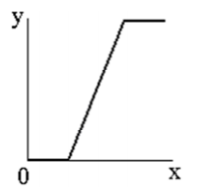
\includegraphics[width=0.22\textwidth]{images/funcLinStreach.png}
\caption{Функция линейного контрастирования изображения}
\label{fig:funcLinStreach}
\end{figure}

\begin{figure}[h!]
\centering
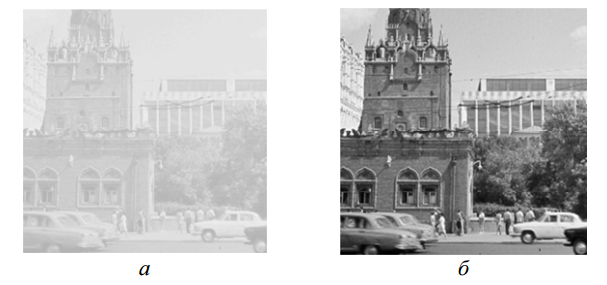
\includegraphics[width=0.8\textwidth]{images/linStreachExample.png}
\caption{ Пример линейного растяжения гистограммы}
\label{fig:exampleLinStreach}
\end{figure}


\section*{Описание схемы распараллеливания}
\addcontentsline{toc}{section}{Описание схемы распараллеливания}

На вход подается одномерный массив пикселей размера $m\cdot n$. Благодаря этому массив хранится линейно в оперативной памяти, что дает нам большое преимущество в распределении определенных блоков между процессами при помощи функции \textbf{MPI\textunderscore Scatterv} (рис.\ref{fig:distrImage}).

\vspace{5mm}

\begin{figure}[h!]
\centering
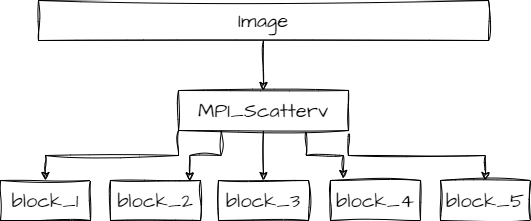
\includegraphics[width=0.8\textwidth]{images/distrImage.png}
\caption{Распределение изображения между 5 процессами.}
\label{fig:distrImage}
\end{figure}

\vspace{5mm}

После того, когда на каждом процессе будет свой участок изображения, нам необходимо найти максимальное и минимальное значение пикселей. Затем при помощи функции \textbf{MPI\textunderscore Allreduce} редуцировать все локальные результаты по операциям \textbf{MPI\textunderscore MAX} и \textbf{MPI\textunderscore MIN} соответсвенно (рис. \ref{fig:allreduce}).

\vspace{5mm}

\begin{figure}[h!]
\centering
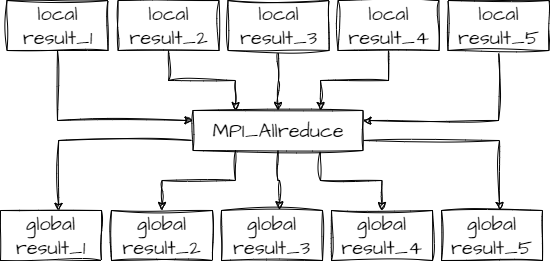
\includegraphics[width=0.8\textwidth]{images/MPI_Allreduce.png}
\caption{Редуцирование 5 процессов.}
\label{fig:allreduce}
\end{figure}

\vspace{5mm}

Следующим этапом будет вызов последовательной версии алгоритма для каждого из процессов, где каждый пиксель будет обработан по формуле, которая была указана ранее (\ref{formulaLinStreach}).

\vspace{2cm}

Самым последним действием будет сбор и объединение полученных локальных изображений при помощи функции \textbf{MPI\textunderscore Gatherv} (рис.\ref{fig:gatherv}).

\vspace{5mm}

\begin{figure}[h!]
\centering
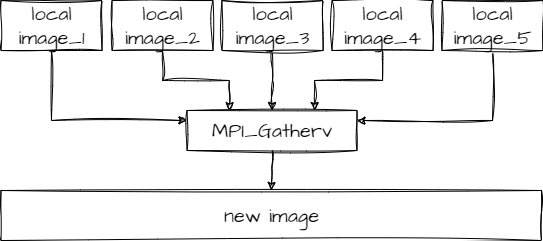
\includegraphics[width=0.8\textwidth]{images/gatherv.png}
\caption{Объединение 5 локальных изображений в результирующее.}
\label{fig:gatherv}
\end{figure}


\section*{Заключение}
\addcontentsline{toc}{section}{Заключение}

В данной лабораторной работе мною были расмотрены и реализованы две версии алгоритма линейного растяжения гистограммы.\newline

За время выполнения работы я получил большой опыт в проектировании, а также последующей разработке и отладке многопроцессорных программ.\newline

Таким образом в заключение можно отметить, что многопроцессорные программы гораздо эффективнее обычных (однопроцессорных), однако их проектирование, разработка и сопровождение на несколько порядков сложнее.

\begin{thebibliography}{99}
    \addcontentsline{toc}{section}{Список литературы}
    
    \bibitem{Starvoitov}
    Получение и обработка изображений на ЭВМ : учебно-методическое пособие / В.В. Старовойтов, Ю.И. Голуб. – Минск : БНТУ, 2018. – 204 с. ISBN 978-985-550-770-4. 
    
    \bibitem{Chaban}
    Чабан Л.Н. Автоматизированная обработка аэрокосмической информации при картографировании геопространственных данных. Учебное пособие. – М.: МИИГАиК, 2013г., - 96 с.
    
    \bibitem{wiki}
    Wikipedia - \url{https://en.wikipedia.org/wiki/Main_Page}
    \end{thebibliography}
    
    

    \section*{Приложение}\label{prog}
    \addcontentsline{toc}{section}{Приложение}
    
    \vspace{5mm}
    
    % \subsubsection*{contrast\textunderscore enhancement.h}
    % \lstinputlisting[language=C++]{code/contrast_enhancement.h}
    
    % \vspace{1cm}
    
    % \subsubsection*{contrast\textunderscore enhancement.cpp}
    % \lstinputlisting[language=C++]{code/contrast_enhancement.cpp}
    
    % \vspace{1cm}
    
    % \subsubsection*{main.cpp}
    % \lstinputlisting[language=C++]{code/main.cpp}
        
\end{document}